\def\pgfsysdriver{pgfsys-dvipdfm.def}
\documentclass[12pt]{beamer}

\usetheme{Warsaw}

%\setbeamertemplate{footline}{}	
\setbeamertemplate{headline}{}
\setbeamertemplate{navigation symbols}{}

\usepackage{color}
\usepackage{xcolor}
\usepackage{indentfirst}
\usepackage[export]{adjustbox}
\usepackage{float}
\usepackage{wrapfig}
\usepackage{setspace}
\usepackage{fontspec}
\usepackage{graphicx}
\usepackage{subcaption}
\usepackage{pgfpages}
\usepackage{amsmath}
\usepackage{bbm}
\usepackage{dsfont}
\usepackage[backend=biber]{biblatex}
\usepackage{xeCJK}
%\addbibresource{bh.bib}
\bibliography{bh}

%\setbeameroption{show notes on second screen=right}
%\setbeamertemplate{note page}[plain]

\addtobeamertemplate{frametitle}{\vspace*{-5pt}}{\vspace*{0pt}}

%\usepackage[scaled=0.95]{helvet}

\renewcommand*{\thefootnote}{[\arabic{footnote}]}

\usefonttheme{professionalfonts}

\setsansfont{Open Sans}[Scale=0.8]
\setCJKsansfont[Scale=0.8]{WenQuanYi Micro Hei}

\setbeamerfont{title}{
	%size={\fontsize{16}{16}}
}

\setbeamerfont{date}{
	family=\fontspec{WenQuanYi Micro Hei}
	%size={\fontsize{50}{50}}
}

\setbeamerfont{note page}{
	%family=\fontspec{WenQuanYi Micro Hei}
	size={\fontsize{14}{14}}
}

\setbeamerfont{note title}{
	size = {\fontsize{12}{12}}
}

\setbeamerfont{institute}{
	%family=\fontspec{Open Sans},
	%size={\fontsize{7}{7}}
}

\setbeamerfont{footnote}{
	size={\fontsize{9}{9}}
}

\setbeamerfont{footline}{
	size={\fontsize{7}{7}}
}

\title{Spectral Clustering of Graphs with the Bethe Hessian}

\author{Alaa Saade\inst{1} \and Florent Krzakala\inst{1,2} \and Lenka Zdeborov\'a\inst{3}}

\institute{
	\inst{1}
	Laboratoire de Physique Statistique, CNRS UMR 8550, \\
  Universit\'e P. et M. Curie Paris 6 et \'Ecole Normale Sup\'erieure,
  24, rue Lhomond, 75005 Paris, France.
	\and
	\inst{2}
	ESPCI and CNRS UMR 7083 Gulliver, 10 rue Vauquelin,Paris 75005
	\and
	\inst{3}
	Institut de Physique Th\'eorique, CEA Saclay and URA 2306, CNRS, 91191 Gif-sur-Yvette, France
}

\date{%  Speaker:\quad 李\,寰
}

\newcommand{\insfig}[2][1]{
	\begin{figure}
		\includegraphics[width=#1\textwidth]{#2.pdf}
	\end{figure}
}
\newcommand{\cin}{c_{\mathrm{in}}}
\newcommand{\cout}{c_{\mathrm{out}}}
\newcommand{\id}{\mathds{1}}

\graphicspath{{figs/}}

\begin{document}
\begin{spacing}{1.3}

\frame{
	\vspace{15pt}
	\titlepage
}
\note{
	\begin{itemize}
		\item NIPS 14
		\item A new method for spectral clustering
		\item Clustering by computing the spectrum of the Bethe Hessian matrix
		\item It illustrates
			\begin{itemize}
				\item relatively better performance
				\item relatively low time complexity	
			\end{itemize}
	\end{itemize}
}

\frame{
	\frametitle{Clustering by the Laplacian $L = D - A$\footnote[frame]{Ulrike Luxburg (2007). A tutorial on spectral clustering. Statistics and Computing,
17(4):395-416.}}
	%\begin{block}{Unnormalized spectral clustering}
	Input: Adjacency matrix $A \in \mathbb{R}^{n\times n}$, number of clusters $q$
	
	\begin{itemize}
		\item $q = 2$
			\begin{itemize}
				\item Cluster by the signs of the 2nd eigenvector of $L$
			\end{itemize}
		\item $q > 2$
			\begin{itemize}
				\item Let $u_1, \cdots, u_q$ be the first $q$ eigenvectors of $L$ %\vspace{5pt}
				\item Let $ U = (u_1, \cdots, u_q) \in \mathbb{R}^{n\times q}$ %\vspace{5pt}
				\item Let $ 
				\begin{pmatrix}
					y_1 \\ \vdots \\ y_n
				\end{pmatrix}
				= U
				$
				%\vspace{5pt}
				\item Cluster the points $y_1, \cdots, y_n \in \mathbb{R}^q$ with $k$-means
			\end{itemize}
	\end{itemize}
	%\end{block}
}
\note{
	\begin{itemize}
		\item Clustering by the Laplacian
	\end{itemize}
}

\frame{
	\frametitle{Clustering by the Adjacency Matrix $A$\footnote[frame]{Avrim Blum, John Hopcroft, and Ravindran Kannan (2016). Foundations of Data Science (pp. 275-281).}}
	\insfig{Spectral_Clustering}
}

\frame{
	\frametitle{Spectral Clustering in Sparse Networks}
	\begin{itemize}
		\item Clustering based on $A$ fails to detect communities
		\vspace{5pt}
		\item Locally tree-like structure
		\vspace{5pt}
		\item Leading eigenvalues of $A$ are dictated by the vertices of highest degree\footnote[frame]{Michael Krivelevich and Benny Sudakov (2003). The largest eigenvalue of sparse
random graphs. Combinatorics, Probability and Computing, 12(01):61-72.}
		\vspace{5pt}
		\item Corresponding eigenvectors are localized around these vertices\footnotemark[\value{footnote}]
	\end{itemize}
}

\frame{
	\frametitle{Clustering by the Non-Backtracking Matrix\footnote[frame]{Florent Krzakala, Cristopher Moore, et al (2013). Spectral redemption in clustering
sparse networks. Proceedings of the National Academy of Sciences, 110(52):20935–20940.}}
	\begin{itemize}
		\item The $2m\times 2m$ non-backtracking matrix $B$
		\[
		B_{(u \to v),(x \to y)} = \begin{cases} 
		1 & \mbox{if $v=x$ and $u \ne y$} \\
		0 & \mbox{otherwise} \, . 
		\end{cases}
		\]
		\item The spectrum of $B$ is not sensitive to high-degree vertices
		%\begin{itemize}
		%	\item A tree contributes zero eigenvalues to the spectrum
		%\end{itemize}
		\item Properties of $B$
			\begin{itemize}
				\item A tree contributes zero eigenvalues to the spectrum
				\item Unicyclic components yield eigenvalues either $1$ or $-1$
			\end{itemize}

	\end{itemize}
}


\frame{
	\frametitle{Stochastic Block Model}
	\vspace{-5pt}
	\begin{itemize}
		\item Stochastic block model
			\begin{itemize}
				\item $q$ groups of vertices with size $n/q$
				\item Each vertex $v$ has a group label $g_v \in \{1, \cdots, q\}$
				\item Adjacency matrix $A$ is generated according to the distribution \vspace{-7.5pt}
				\[
					\Pr[A_{u,v}=1] = \begin{cases}	
						\cin / n & g_u = g_v \\
						\cout / n & g_u \neq g_v 
					\end{cases},
					\mbox{where}\ \cin > \cout
				\]
			\end{itemize}
		\item \vspace{-5pt} Average degree $c = (\cin + \cout)/2$ \hspace{1pt} when $q = 2$
			%\begin{itemize}
			%	\item $L = D - A \approx c\id - A$
			%	\item Clustering by the second largest eigenvector of $A$
			%\end{itemize}
		\item $G$ becomes sparse when $n$ is large
			%\begin{itemize}
			%	\item Spectral clustering by $A$ fails
			%\end{itemize}
	\end{itemize}
}

\frame{
	\frametitle{Spectrum of $A$ and $B$}
%	\vspace{-5pt}
	\vspace{-5pt}
	\begin{figure}
		\makebox[\linewidth][c]{
		\begin{subfigure}[H]{0.45\textwidth}
			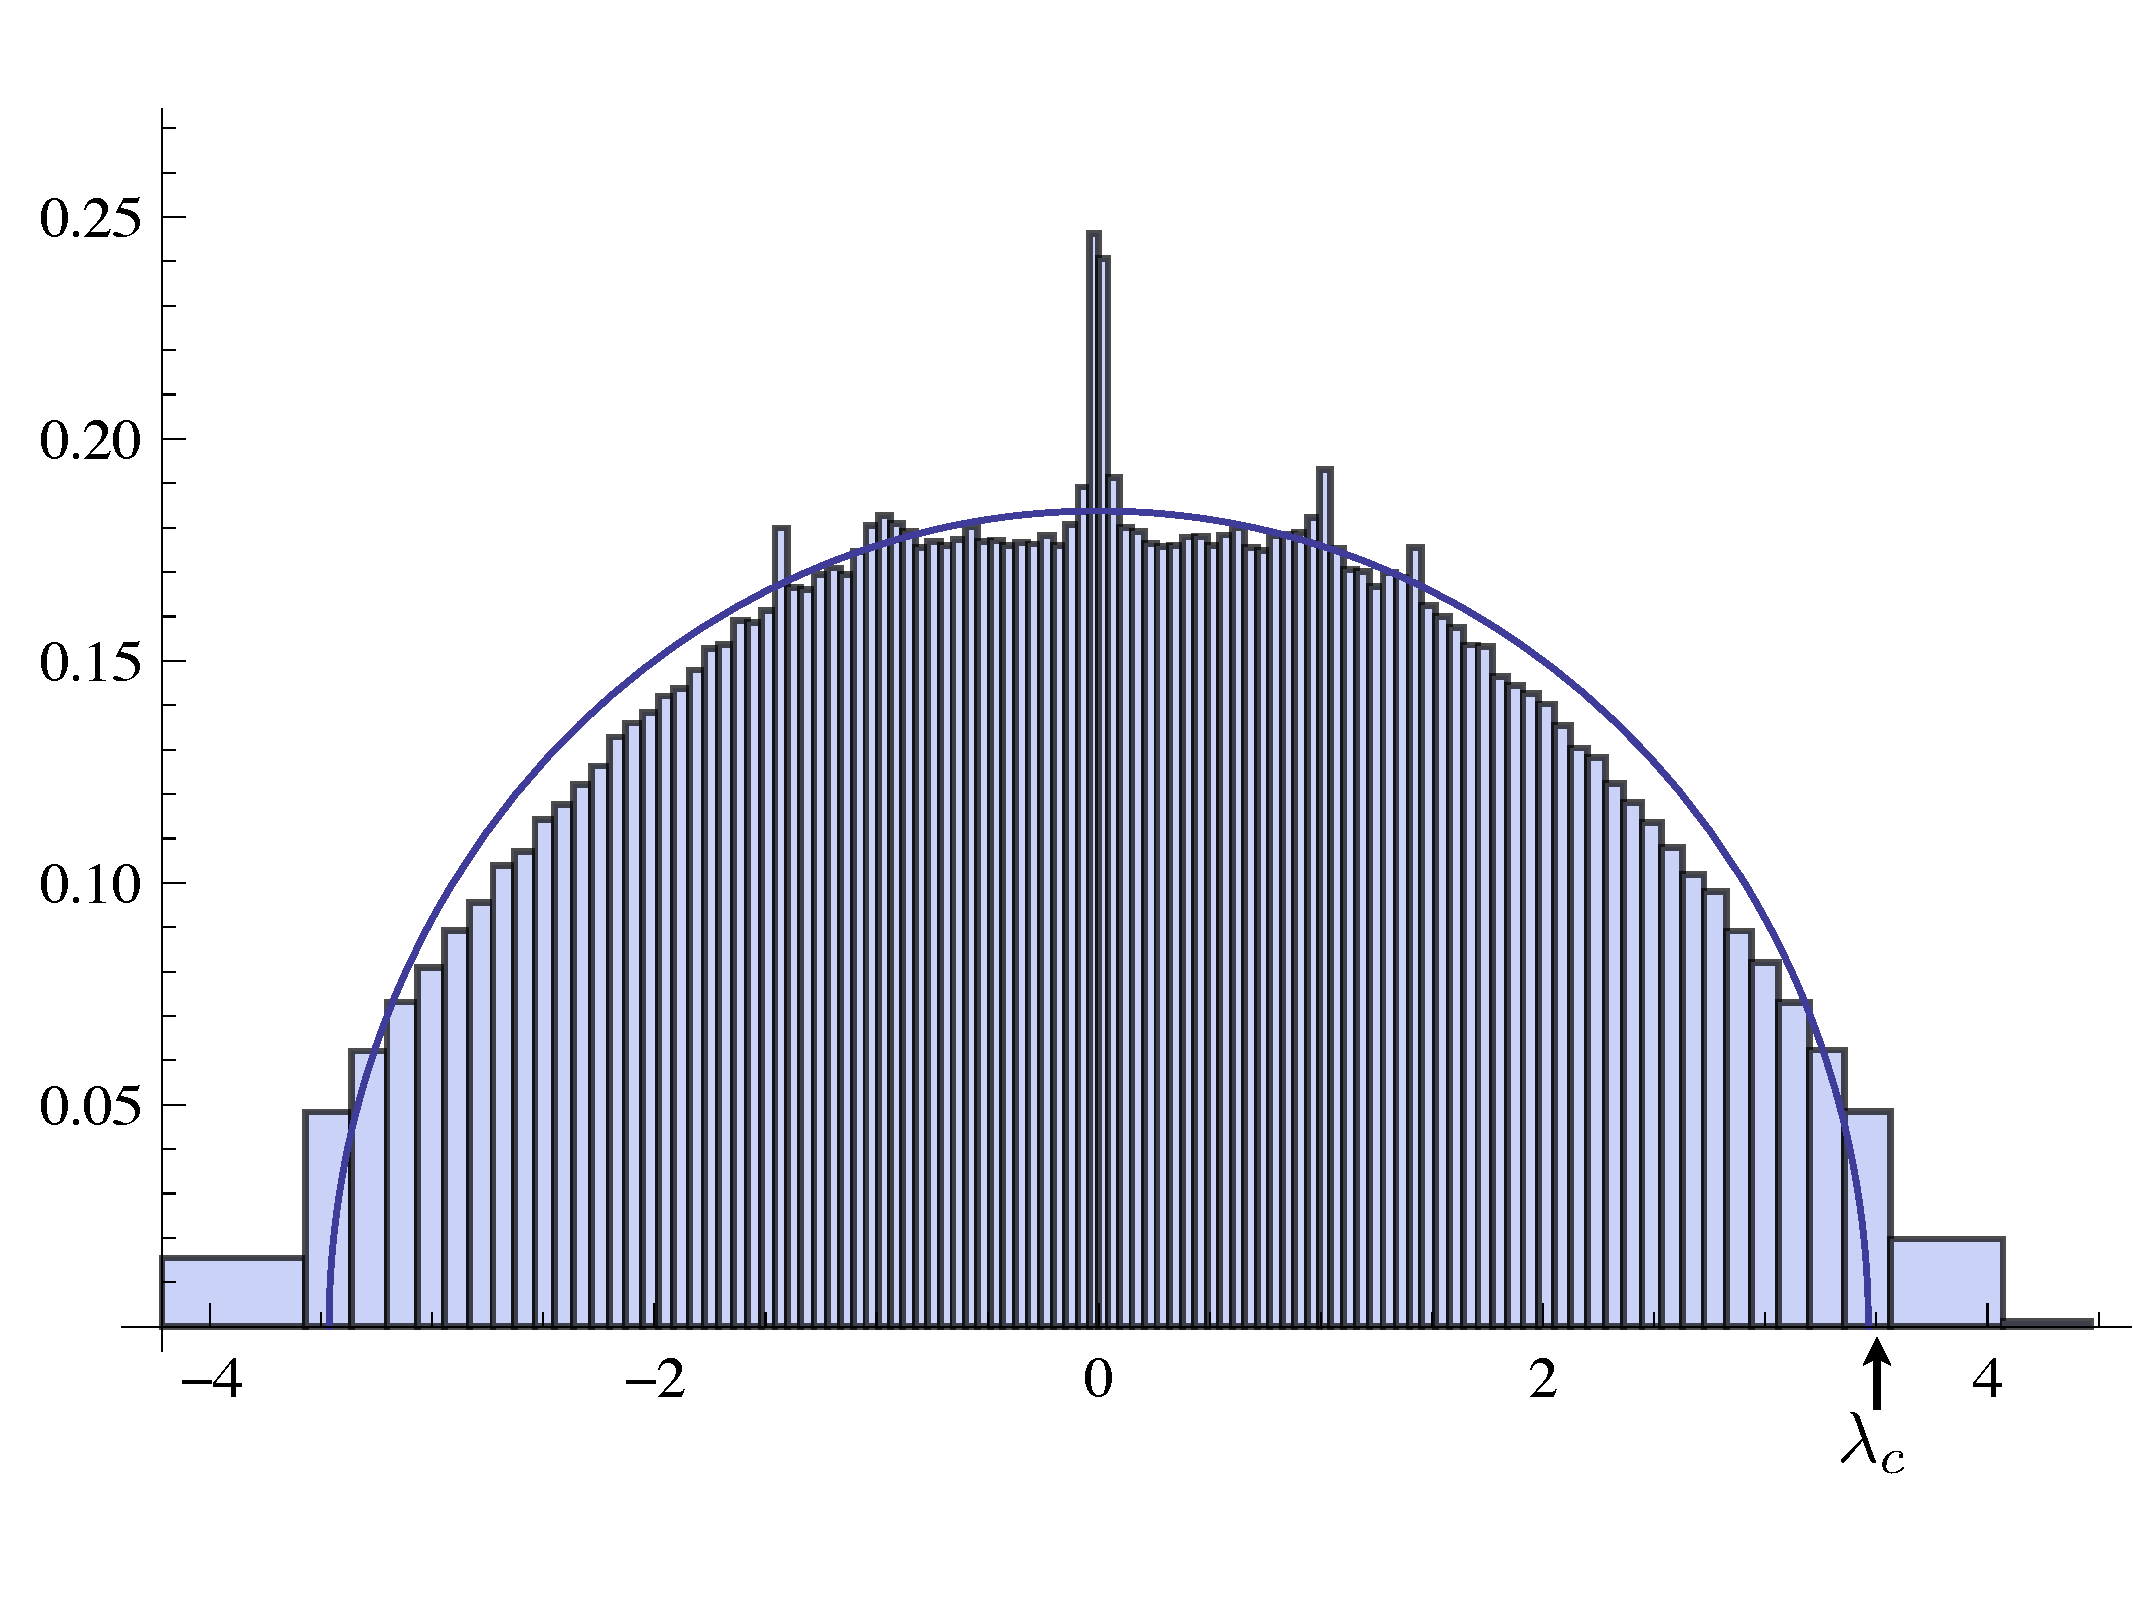
\includegraphics[width=1\textwidth]{EXP1}
			\label{exp1}
			\caption{The spectrum of $A$}
		\end{subfigure}
		\hspace{20pt}
		\begin{subfigure}[H]{0.45\textwidth}
			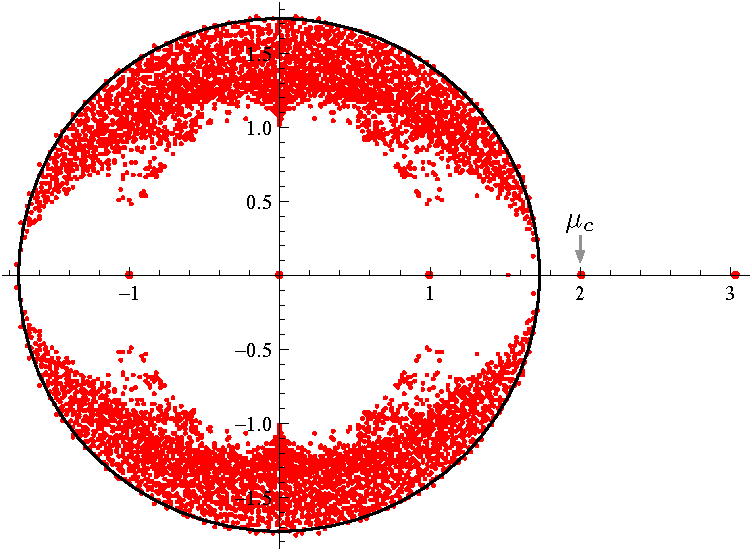
\includegraphics[width=1\textwidth]{EXP2}
			\label{exp2}
			\caption{The spectrum of $B$}
		\end{subfigure}
		}
		%\caption{The spectrum of $A$ (left) and $B$ (right)}
	\end{figure}
	\begin{itemize}
		\item $n = 4000$, $\cin = 5$, $\cout = 1$
		\item The radius of the bulk
			\begin{itemize}
				\item For $A$, $2\sqrt{c} = 3.46$ 
				\item For $B$, $\sqrt{c} = \sqrt{3}$
			\end{itemize}
	\end{itemize}
}

\frame{
	\frametitle{Experiments $n = 10^5$}	
	\begin{figure}
		\makebox[\linewidth][c]{
		\begin{subfigure}[H]{0.45\textwidth}
			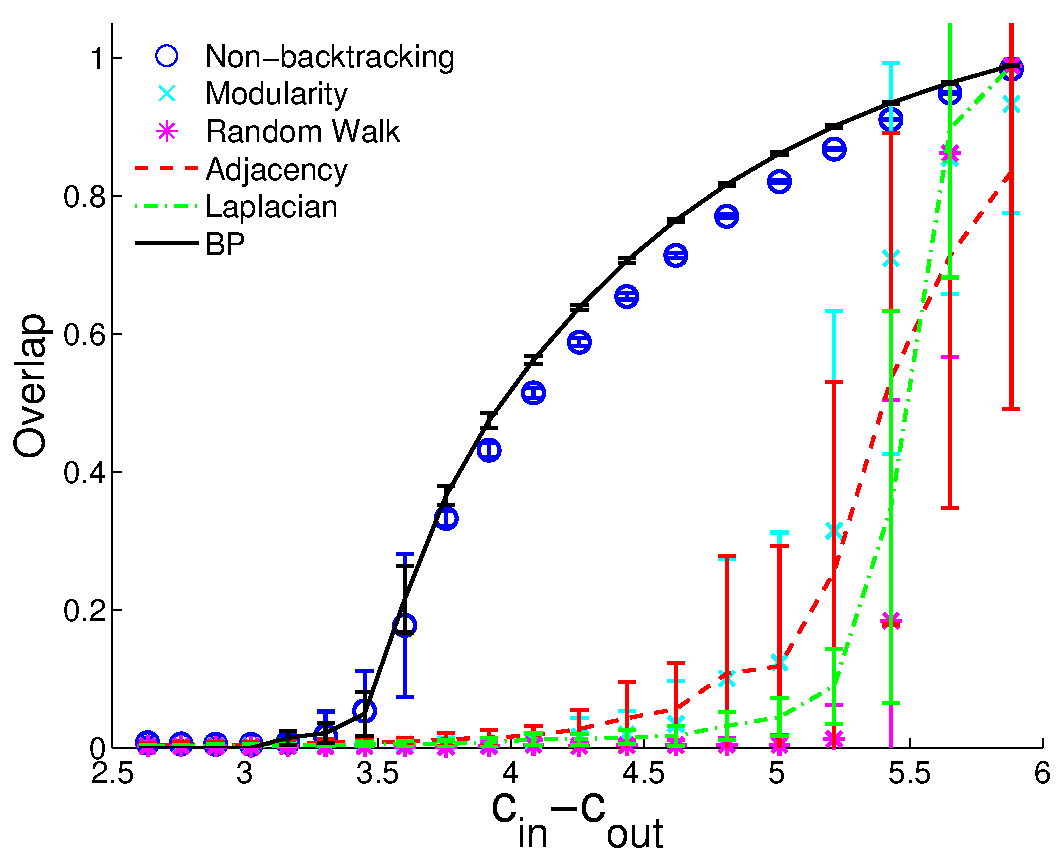
\includegraphics[width=1\textwidth]{EXP3}
			%\caption{The first 3 eigenvalues of $B$}
		\end{subfigure}
		\quad
		\begin{subfigure}[H]{0.45\textwidth}
			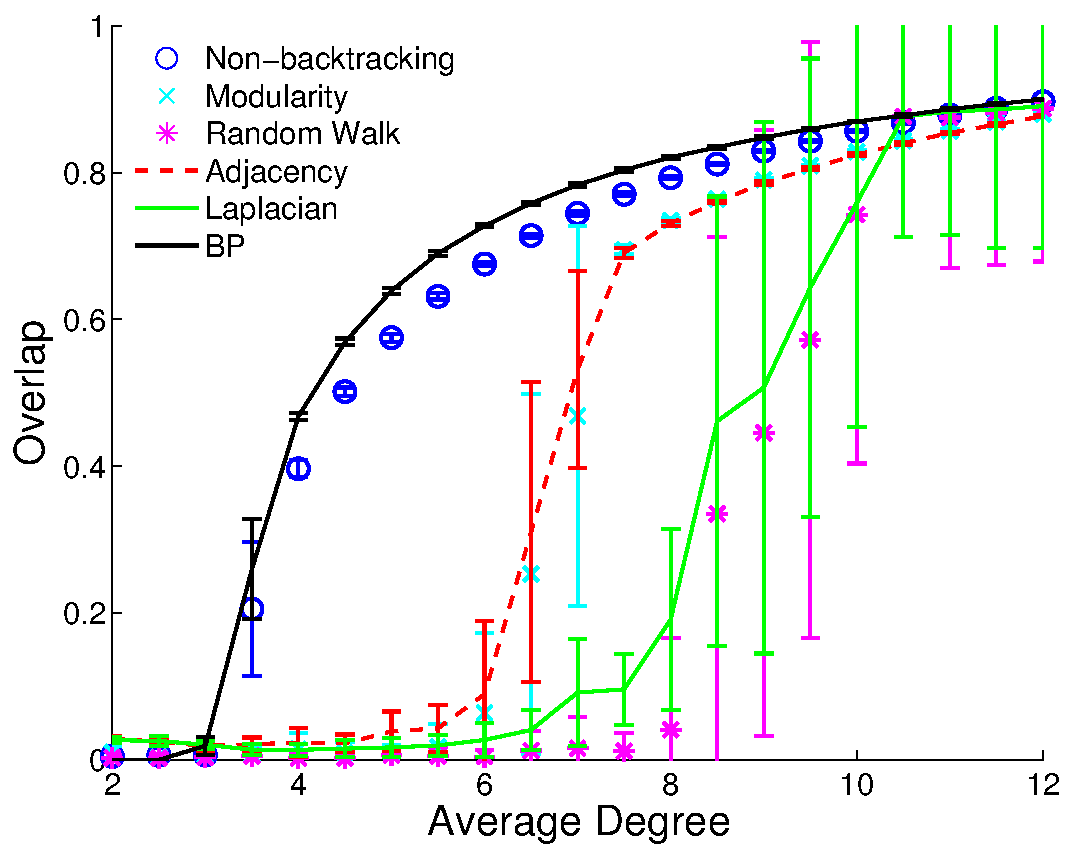
\includegraphics[width=1\textwidth]{EXP4}
		\end{subfigure}
		}
		%\caption{The accuracy of spectral clustering based on different matrices}
	\end{figure}
	\vspace{-5pt}
	\begin{itemize}
		%\item $n = 10^5$
			%\begin{itemize}
			%	\item On the left, set $c = 3$ and vary $\cin - \cout$
			%	\item On the right, set $\cout/\cin = 0.3$ and vary $c$
			%\end{itemize}
		\item $\mbox{Overlap} \triangleq
        \left( \frac{1}{n} \sum_u \delta_{g_u , \tilde{g}_u} -
          \frac{1}{q}\right) \Big{/} \left( 1 -  \frac{1}{q} \right)
$
		\vspace{5pt}
		\item Theoretical threshold\footnote[frame]{Elchanan Mossel, Joe Neeman, and Allan Sly (2012). Stochastic block models and
reconstruction. arXiv preprint, arXiv:1202.1499.} $\approx 3.46$
	\end{itemize}
}

\frame{
	\frametitle{Detecting Number of Clusters}
	\begin{figure}
		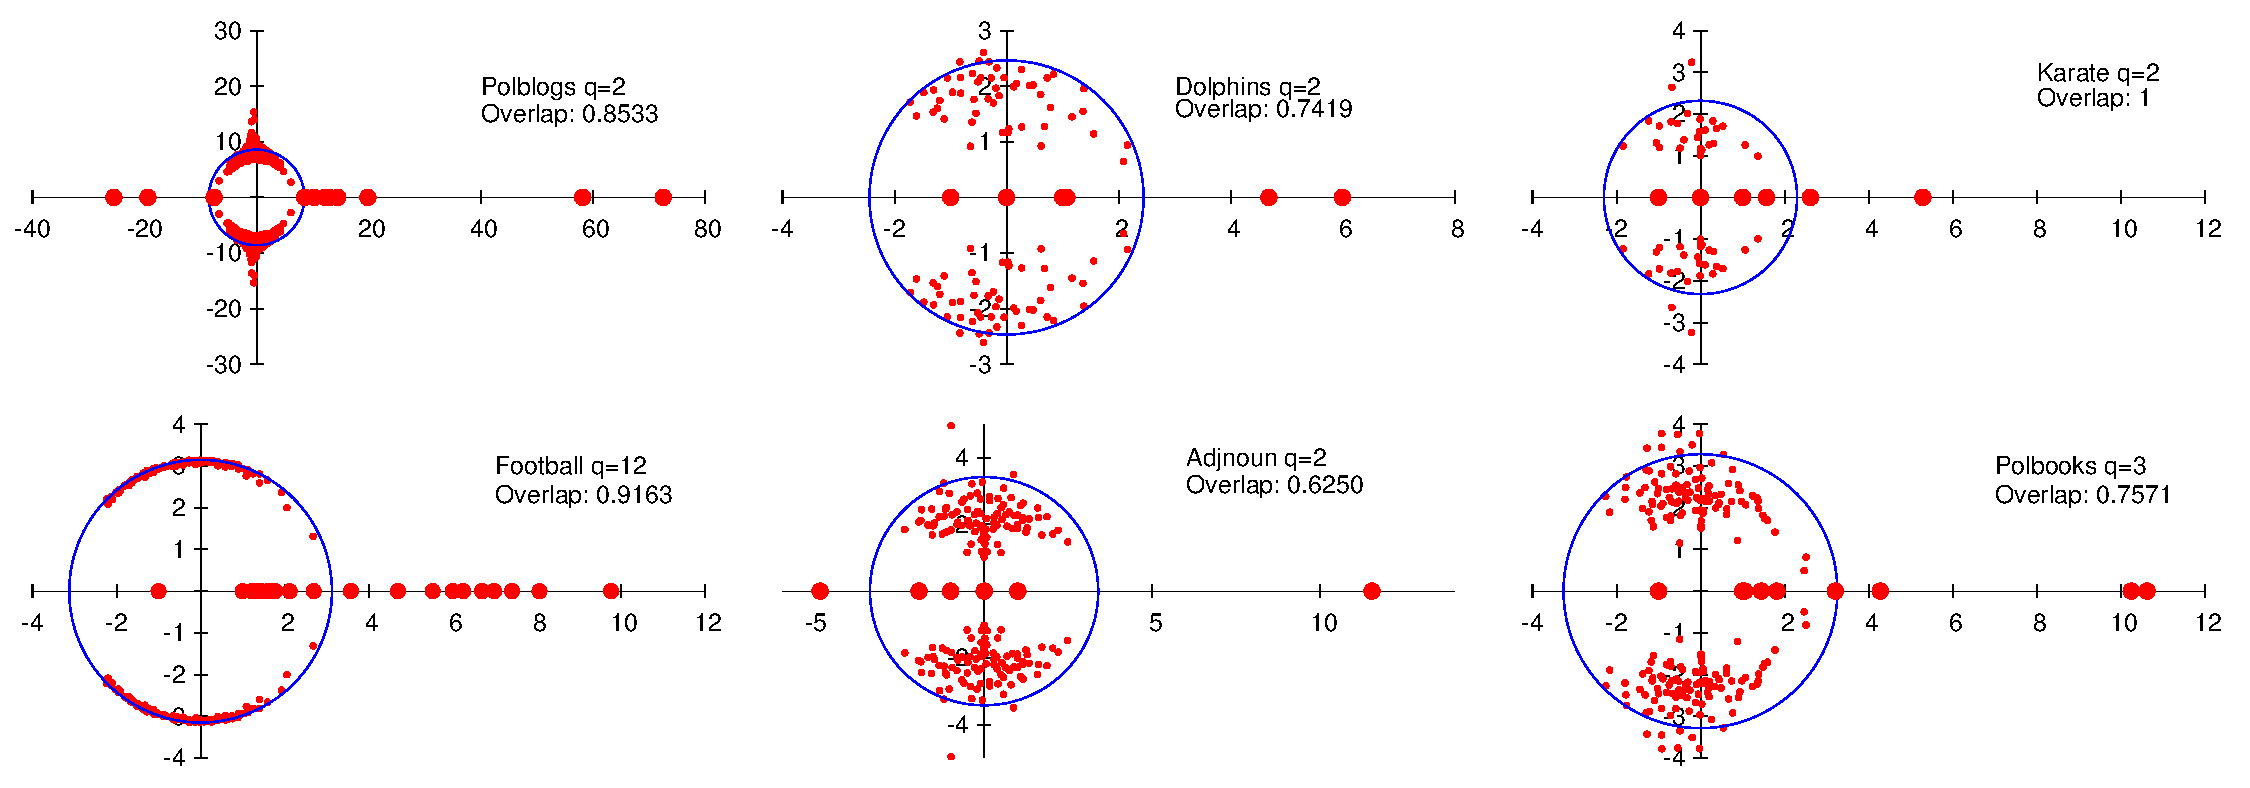
\includegraphics[width=1\textwidth]{DNOC}
		%\hspace*{8cm}
		\begin{itemize}
			\item Each circle's radius is $\sqrt{\rho(B)}$
			\item The number of real eigenvalues outside the circle indicates the number $q$ of clusters
		\end{itemize}
	\end{figure}
}


\frame{
	\frametitle{Reducing the Computational Complexity}
	%\vspace{-3.5pt}
	\begin{itemize}
		\item All eigenvalues $\lambda$ of $B$ not $\pm 1$ are the roots of the equation\footnote[frame]{Omer Angel, Joel Friedman, and Shlomo Hoory (2015). The non-backtracking spectrum of the universal cover of a graph. Trans. Amer. Math. Soc., 367(6):4287-4318.}
		\vspace{-10pt}
		\begin{equation} 
			\label{eq:ihara}
			\det \left[ \lambda^2 \id - \lambda A + (D-\id) \right] = 0 \,
		\end{equation}
		\item \vspace{-10pt} By the first companion linearization\footnote[frame]{Francoise Tisseur and Karl Meerbergen (2001). The quadratic eigenvalue problem. SIAM
Review, 43(2):235-286.}, roots of eq.~(\ref{eq:ihara}) are eigenvalues of \vspace{-10pt}
		\begin{equation}
			\label{eq:2nby2n}
			B' = \begin{pmatrix}
			0 & D-\id \\
			-\id & A
			\end{pmatrix}\quad \quad \quad \quad \nonumber
		\end{equation}
		\item \vspace{-2.5pt} Clustering by a $2n\times 2n$ matrix rather than a $2m\times 2m$ one
	\end{itemize}
}

\frame{
	\frametitle{The Bethe Hessian Matrix}
	\vspace{-9pt}
	\begin{itemize}
		\item All eigenvalues $\lambda$ of $B$ not $\pm 1$ are the roots of the equation
		\vspace{-10pt}
		\begin{equation} 
			\label{eq:ihara}
			\det \left[ \lambda^2 \id - \lambda A + (D-\id) \right] = 0 \,
			\tag{1}
		\end{equation}
	\item The Bethe Hessian matrix $H(r)$
			\[
				H(r):=r^2\id-rA+(D - \id) %\quad \quad  \quad \quad
			\]
			\item $\forall$ real eigenvalue $\lambda$ of $B$, $H(\lambda)$ has a eigenvalue 0
			\begin{itemize}
				\item $H(\lambda)$'s null space \hspace{2pt} $\longleftrightarrow$ \hspace{2pt} $B$'s eigenvector corresponding to $\lambda$
				\item Let $r_c = \sqrt{\rho(B)}$
				\item Eigenvectors of $H(r_c)$'s negative eigenvalues reveal clustering
			\end{itemize}
	\end{itemize}
}

\frame{
	\frametitle{Spectrum of $B$ and $H(r)$}
	\vspace{-20pt}
	\begin{wrapfigure}{L}{0.55\textwidth}
		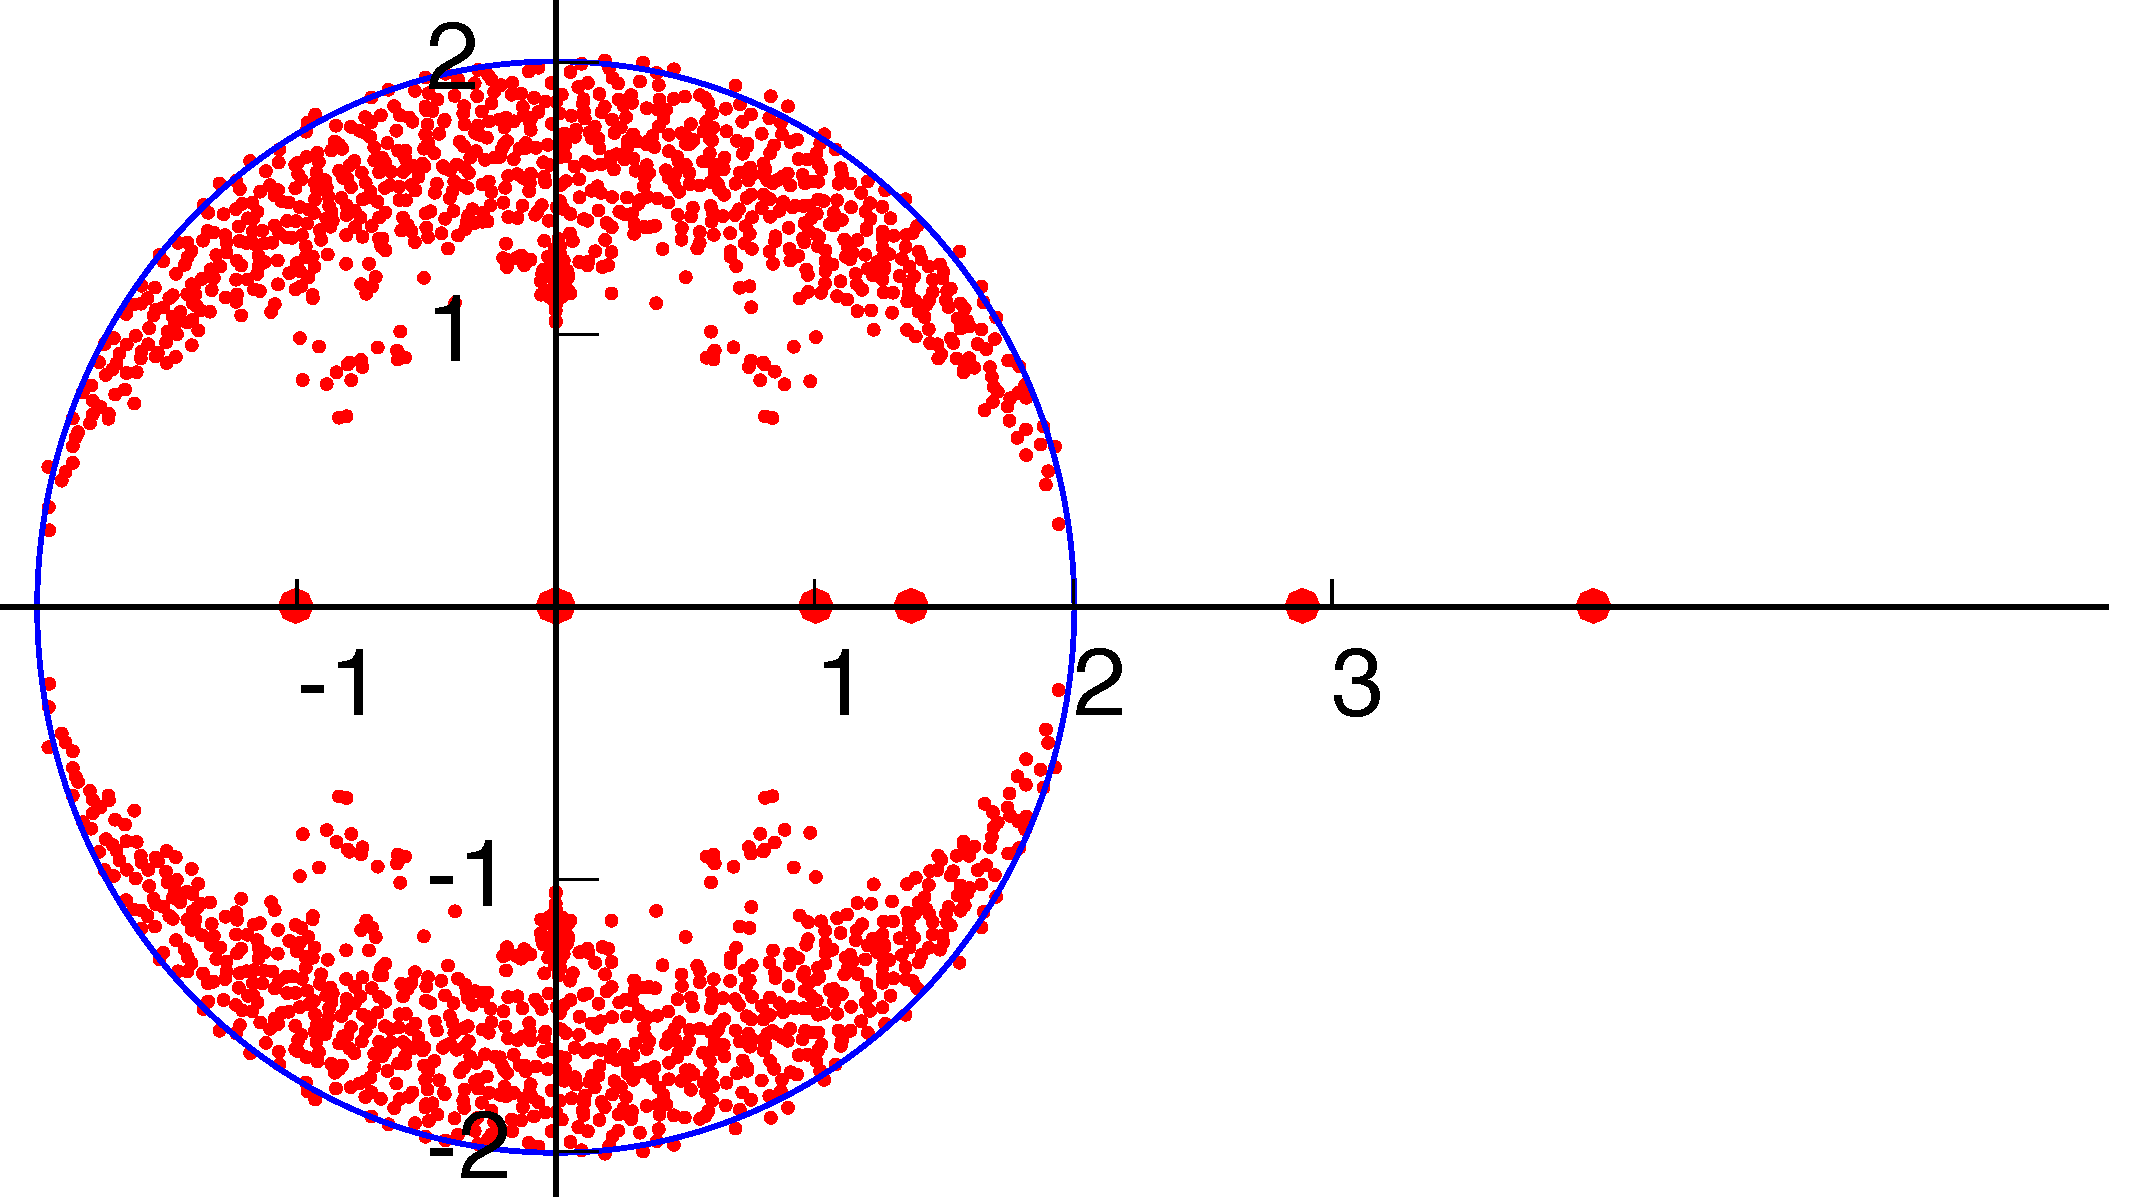
\includegraphics[width=0.5\textwidth]{1000}
	\end{wrapfigure}
	\quad \\[2.5pt]
	Stochastic block model
	\begin{itemize}
		\item $n = 10^4$
		\item $c = 4$
		\item $\cout / \cin = \frac{1}{7}$
	\end{itemize}
	\quad \\[5pt]
	\insfig{AE}
}

\frame{
	\frametitle{Experiments}
	\insfig{EXB1}
	\insfig[0.8]{EXB2}
}

\frame{
	\frametitle{Conclusions and Perspectives}
	\begin{itemize}
		\item Comparing to non-backtracking clustering
			\begin{itemize}
				\item $H(r_c)$ is $n\times n$ symmetric, while $B'$ is $2n\times 2n$ non-symmetric
				\item Need to compute $\rho(B)$ to calculate $r_c = \sqrt{\rho(B)}$
					\begin{itemize}
						\item By solving quadratic eigenproblem~(\ref{eq2}) using a SLP algorithm\footnote[frame]{Axel Ruhe (1973). Algorithms for the nonlinear eigenvalue problem. SIAM Journal on
Numerical Analysis, 10(4):674–689.} \vspace{-5pt}
\begin{equation}
	\label{eq2}
	\det{H(\lambda)} = \det{\left[\lambda^2\id-\lambda A+(D-\id)	\right]} = 0 \quad \quad %\quad %\quad
\end{equation}
			\end{itemize}
		\end{itemize}
		\item \vspace{-5pt} Detecting the communities in sparse network
			\begin{itemize}
				\item All the way down to the threshold in SBM
			\end{itemize}
		\item The number of negative eigenvalues indicating the number of clusters
	\end{itemize}
}

\begin{frame}
	\Huge{\centerline{The End}}
\end{frame}

%\begin{thebibliography}{9}
%\bibitem{ClFi07}
%J.~Clark and R.~Fierro, ``Mobile robotic sensors for perimeter detection and
%  tracking,'' \emph{ISA Trans.}, vol.~46, no.~1, pp. 3--13, 2007.
%\end{thebibliography}

\end{spacing}
\end{document}